\section{Statistical analysis}
%
%%%%%%%%%%%%%%%%%%%%%%%%%%%%%%%%%%%%%%%%%%%%%%%%%%%%%%%%%%%
\subsection{Data} \label{s_sect:data}
%
%%%%%%%%%%%%%%%%%%%%%%%%%%%%%%%%%%%%
\subsubsection{Outcomes} \label{ss_sect:outcome}
%
On the one hand, the outcome for the \textbf{judgment task} was obtained following the procedure outlined in sections \ref{ss_sect:proc} and \ref{ss_sect:expset}, with the total number of judgments per procedure detailed in Table \ref{tab:allocation}.

On the other hand, the outcome from the \textbf{transcription task} was obtained following a two step procedure \citep{Boonen_et_al_2021}. First, we aligned the participant's orthographic transcriptions, at the utterance level, in a column-like grid structure similar to the one presented in Table \ref{tab:align_example}. This step was repeated for every one of the $6400$ transcriptions\footnote{\label{foot:doe}under DoE literature, the design corresponds to $32$ experimental units with $10$ replicates each, making a total of $320$ experimental runs. Moreover, we register $20$ duplicates (transcriptions) for each run, making a total of $6400$ transcriptions.} (see Section \ref{s_sect:JandT}). Lastly, we computed the entropy measure of the aligned transcriptions as in \citet{Shannon_1948}: 
%
\begin{equation} \label{eq:entropy}
	H = H(\pmb{p}) = \frac{-\sum_{i=1}^{n} p_{i} \cdot \log_{2}(p_{i})}{\log_{2}(N)}
\end{equation}
%
where $n$ denotes the number of word occurrences, $p_{i}$ the probability of the word occurrence, and $N$ the total number of aligned transcriptions per utterance.
%
\begin{table}[h!]
	\centering
	\begin{tabular}{|| c | ccccc || } 
		\hline
		Transcription & \multicolumn{5}{c ||}{Utterance} \\ [0.5ex]
		\cline{2-6}
		number & 1 & 2 & 3 & 4 & 5 \\ [0.5ex] 
		\hline\hline
		1 & de & jongen & ziet & een & kikker \\ 
		  & the & boy & see & a & frog \\ 
		\hline
		2 & de & jongen & ziet & de & [X] \\
		  & the & boy & sees & the & [X] \\ 
		\hline
		3 & de & jongen & zag & [B] & kokkin \\
		  & the & boy & saw & [B] & cook \\ 
		\hline
		4 & de & jongen & zag & geen & kikkers \\
		  & the & boy & saw & no & frogs \\ 
		\hline
		5 & de & hond & zoekt & een & [X] \\
		  & the & dog & searches & a & [X] \\ 
		\hline
		Entropy & $0$ & $0.3109$ & $0.6555$ & $0.8277$ & $1$ \\
		\hline
		\multicolumn{4}{l}{\footnotesize{[B] = blank space, [X] = unidentifiable word}}
	\end{tabular}
	\caption{Example of five aligned transcriptions and its corresponding entropy calculations. Extracted from \citet{Boonen_et_al_2021}, and slightly modified with illustrative purposes.}
	\label{tab:align_example}
\end{table}
%

Entropy was used as an objective measure of SI, i.e. a quantification of (dis)agreement between listeners' transcriptions. Utterances yielding a high degree of agreement between transcribers were considered highly intelligible, and therefore registered a lower entropy $\left( H \rightarrow 0 \right)$. In contrast, utterances yielding a low degree of agreement were considered as exhibiting low intelligibility, and therefore registered a higher entropy $\left( H \rightarrow 1 \right)$ \citep{Boonen_et_al_2021, Faes_et_al_2021}. 

Using Table \ref{tab:align_example}, we exemplify the entropy calculation for utterances $2$, $4$ and $5$, which represent relevant scenarios for the procedure. Notice that every calculation considers five transcriptions in total ($N=5$). 

For the second utterance, we observe that four transcriptions identify it with the word \textit{jongen}, while the last with the word \textit{hond}. Therefore, we registered two word occurrences ($n=2$), with probabilities $\pmb{p} = (p_{1}, p_{2}) = (4/5, 1/5)$, and an entropy measure equal to:
%
\begin{align*}
	H &= \frac{-\sum_{i=1}^{2} p_{i} \cdot \log_{2}(p_{i})}{\log_{2}(5)} \\
	%
	&= \frac{- \left[ 0.8 \log_{2}(0.8) + 0.2 \log_{2}(0.2) \right] }{\log_{2}(5)} \\
	%
	&\approx 0.3109
\end{align*} 
%
For the fourth utterance, we observe that two transcriptions identify it with the word \textit{een}, one with \textit{de}, one with \textit{geen}, and one with a blank space [B]. Notice the blank space was not expected in such position, therefore, it was considered as a different word occurrence. As a result, the scenario had four word occurrences ($n=4$), with probabilities $\pmb{p} = (p_{1}, p_{2}, p_{3}, p_{4}) = (2/5, 1/5, 1/5, 1/5)$, and an entropy measure equal to:
%
\begin{align*}
	H &= \frac{-\sum_{i=1}^{4} p_{i} \cdot \log_{2}(p_{i})}{\log_{2}(5)} \\
	%
	&= \frac{- \left[ 0.4 \log_{2}(0.4) + 3 \cdot 0.2 \log_{2}(0.2) \right] }{\log_{2}(5)} \\
	%
	&\approx 0.8277
\end{align*} 
%
Finally, for the fifth utterance, we observe that all of the  transcriptions identify it with different words. Notice we consider the unidentifiable word [X] in the second transcription, as being different from the one in the last. This is done to avoid the artificial reduction of the entropy measure, as [X] values already indicate the lack of intelligibility of the word. Therefore, we registered five word occurrences ($n=5$), with probabilities $\pmb{p} = (p_{1}, \dots, p_{5}) = (1/5, \dots, 1/5)$, and an entropy measure equal to:
%
\begin{align*}
	H &= \frac{-\sum_{i=1}^{5} p_{i} \cdot \log_{2}(p_{i})}{\log_{2}(5)} \\
	%
	&= \frac{- 5 \cdot 0.2 \log_{2}(0.2) }{\log_{2}(5)} \\
	%
	&= 1
\end{align*} 
%
%
%%%%%%%%%%%%%%%%%%%%%%%%%%%%%%%%%%%%
\subsubsection{Covariates} \label{ss_sect:covariates}
%
The characteristics of the selected children is detailed in Table \ref{tab:children_char} from Appendix \ref{appA:char}. The table includes all the variables used for the matching procedure in Section \ref{s_sect:children}, and additionally, shows the child's etiology, i.e. the cause of their hearing impairment, and their post-implant pure tone average (PTA), i.e. the child's subjective hearing sensitivity, aided and unaided by their hearing apparatus. No other variables are included as no known additional comorbidities, beside their hearing impairment, is suspected.

From the table, \textcolor{red}{describe summaries from the table.}
%
%
%%%%%%%%%%%%%%%%%%%%%%%%%%%%%%%%%%%%
\subsubsection{Pre-processing} \label{ss_sect:preproc}
%
Besides the exclusion of corrupted observations, e.g. no available rating, no other experimental run nor duplicate was eliminated before the modeling process. This decision departs from what it is observed in previous research, e.g. \citet{Boonen_et_al_2020} decided to eliminate "outlying" observations based on misfit analysis \citep{Lesterhuis_2018}, while \citet{vanDaal_2020} and \citet{Boonen_et_al_2021} did the same based on univariate outlier analysis. 

For the case of misfit analysis, we argue that such procedures cannot be used without caution. The literature points out that in the context of CJ, these statistics are always relative, i.e. they depend on other stimulus and judges included in the assessment \citep{Pollitt_2012a, Pollitt_2012b}. Moreover, they have been proven to be less sensitive, as they are calculated with a low number of judgments per representation \citep{Pollitt_2012a}. 

On the other hand, for the case of univariate outlier analysis, we argue that outlying observations are interesting cases to analyze \citep{McElreath_2020}, and usually they cannot be identified properly outside the context of a full model \citep{McElreath_2020}, i.e. what can behave as an outlier based on a univariate analysis, can behave as expected under the appropriate model. 

Considering the previous, if we still manage to identify outlying observations within the context of the proposed models (see Section \ref{s_sect:models}), the researcher would rather make the model robust against their influence.
%
%
%%%%%%%%%%%%%%%%%%%%%%%%%%%%%%%%%%%%%%%%%%%%%%%%%%%%%%%%%%%
\subsection{Model estimation} \label{s_sect:estimation}
%
The models proposed in sections \ref{s_sec:evaluation} and \ref{s_sect:models} will be estimated under the Bayesian framework\footnote{see \citet{Rivera_2021} (p. 11-13, 15-27) for a detailed description of its benefits and shortcomings.}. More specifically, we will use the Hamiltonian Monte Carlo algorithm (HMC) \cite{Duane_et_al_1987, Betancourt_et_al_2013, Neal_2012}. The software package that will provide us with the HMC machinery is \texttt{Stan} \cite{Stan_2020}, while we will use \texttt{R} \cite{R_2015, RStan_2020}, and its integration packages, to analyze its outputs.
%
%
%%%%%%%%%%%%%%%%%%%%%%%%%%%%%%%%%%%%%%%%%%%%%%%%%%%%%%%%%%%
\subsection{Model selection} \label{s_sect:model_sel}
%
Following the successful and comprehensive analysis in \citet{vanDaal_2020} and \citet{Lesterhuis_2018}, the current research will also use the Information-Theoretic Approach (ITA) \citep{Anderson_2008, Chamberlain_1965} for the selection of competing models. The approach considers three steps: (1) state our hypothesis into statistical models, (2) select among competing models, and (3) make inferences based on one or multiple models.

First, for the translation of our working hypotheses into statistical models, we will use Directed Acyclic Graphs (DAG) and probabilistic programming \citep{Jaynes_2003}. A DAG is the simplest representation of a Graphical Causal Model (GCM), a heuristic model that contains information not purely statistical, but unlike a detailed statistical model, it allow us to deduce which variable relationships can provide valid causal inferences \citep{Hernan_et_al_2020, McElreath_2020}. In summary, a DAG is a reasonable way to state our hypothesis, and make our assumption more transparent. However, abide by the \textit{no-free lunch} rule, the causal inferences produced under the DAG will only be valid if the assumed DAG is correct. In contrast, the probabilistic programming will serve as the algebraic formalist to define our statistical models.

Second, to select among competing models, we will use the Widely Applicable Information Criterion (WAIC) \citep{Watanabe_2013}, and the Pareto-smoothed importance sampling cross-validation (PSIS) \citep{Vehtari_et_al_2021}\footnote{\citet{vanDaal_2020} used the Akaike’s Information Criterion (AIC) \citep{Akaike_1974} with similar purposes.}. Two reasons justify our decision. First, both criteria allow us to embrace the full flexibility and information of our bayesian implementation (outlined in Section \ref{s_sect:estimation}). Last, and more important, both criteria provide us with the best approximations for the out-of-sample (cross-validated) deviance \citep{McElreath_2020}, where the deviance is the best approximation for the Kullback-Liebler (KL) divergence \citep{Kullback_et_al_1951}, i.e. a measure of how far a model is from describing the \textit{true} distribution of our data\footnote{also defined as a model's \textit{measure of the relative distance from perfect (predictive) accuracy} \citep{McElreath_2020}.}. \citet{McElreath_2020} points out that is a rather benign characteristic of the model's selection procedure, that we do not need the KL divergence absolute value, as the \textit{true} distribution of our data is not available (otherwise, we would not need a statistical model). But rather, using the deviance difference between competing models, we can measure which model is the farthest from perfect (predictive) accuracy of our data\footnote{for the intuition and the detailed derivation of the argument see \citet{McElreath_2020} (p. 202-211)}.

Finally, considering the evidence provided by the previous step, we proceed to make inferences based on one or multiple models.
%
%
%%%%%%%%%%%%%%%%%%%%%%%%%%%%%%%%%%%%%%%%%%%%%%%%%%%%%%%%%%%
\subsection{Model evaluation} \label{s_sec:evaluation}
%
Considering the objectives outlined in Section \ref{seq:rq}, we will evaluate seven models that serve different, but interrelated purposes:
\begin{enumerate} \itemsep1pt
	\item[(1)] a measurement error model for entropy
	\item[(2)] a measurement model for: 
	\begin{enumerate} \itemsep1pt
		\item absolute holistic judgment (HJ)
		\item dichotomous comparative judgment (CJ-D)
		\item ordinal comparative judgment (CJ-O)
	\end{enumerate}
	\item[(3)] a full integrating model for: 
	\begin{enumerate} \itemsep1pt
		\item models (1) and (2a)
		\item models (1) and (2b)
		\item models (1) and (2c)
	\end{enumerate}
\end{enumerate} 
%

\textcolor{blue}{Model (1) will allow us to construct the \textit{most objective} measure of a child's SI ranking, and to test some research hypothesis of our interest. 
%
The second set of models (2a, 2b, 2c) will allow us to provide preliminary evidence on the reliability and validity of the rating procedures. For the reliability, We will compare 
%
the direction, magnitude, and quality of inference of the same research hypothesis outlined for Model (1), in the newly estimated models.
}
%
%
%%%%%%%%%%%%%%%%%%%%%%%%%%%%%%%%%%%%
\subsubsection{validity}
%
\textcolor{red}{(in process)}

\begin{comment}
	correlate latent scores (from different methods) with entropy measures (see research proposal)
	
	\textbf{critique:} What about decision statements or think at loud rating process? (is it possible), \citet{Lesterhuis_2018} has shown their usefulness, while \citet{Boonen_et_al_2020} signals the need to know about the inner working of judgment processes.
\end{comment}
%
%
%%%%%%%%%%%%%%%%%%%%%%%%%%%%%%%%%%%%
\subsubsection{reliability}
%
\textcolor{red}{(in process)}

\begin{comment}
	compare the Scale Separation Reliability (SSR, an inter-rater reliability measure), coming from CJ methods, with others for other methods
	
	- No intra-rater reliability, also known as test-retest reliability (Verhavert_2018, Reliability_wiki_2022) 
	- No Inter-method reliability,  assesses the degree to which test scores are consistent when there is a variation in the methods or instruments used (Verhavert_2018, Reliability_wiki_2022) 
	- No comparison of SSR vs the true correlation of the latent scale and entropy measures 
	* Justification: (Verhavert_2018, p. 156) " simulation studies could resolve the inconclusiveness regarding the SSR as a correlation with the truth."
\end{comment}
%
%
%%%%%%%%%%%%%%%%%%%%%%%%%%%%%%%%%%%%
\subsubsection{efficiency (time)}
%
\textcolor{red}{(in process)}

\begin{comment}
	time needed for each judgement based on method from (Coertjens_et_al_2017).
	
	statistical efficiency has been researched on \citet{Leijon_et_al_2019} and \citet{Pritikin_2020} for the bayesian dichotomous BTL model and the ordinal BTL model, respectively.
\end{comment}
%
%
%%%%%%%%%%%%%%%%%%%%%%%%%%%%%%%%%%%%%%%%%%%%%%%%%%%%%%%%%%%
\subsection{Models and hypothesis} \label{s_sect:models}
%
\textcolor{blue}{}
%
%
%%%%%%%%%%%%%%%%%%%%%%%%%%%%%%%%%%%%
\subsubsection{Measurement error model for entropy} \\
%
, e.g. if a statistical difference in SI between children with different hearing status, controlling for some other confounding factors

As it is described in Section \ref{ss_sect:outcome}, our data set is composed of $320$ entropy measures, nested within $32$ children with $10$ replicates per child. Each entropy measure was bounded in the continuum $[0,1]$, as expected from equation (\ref{eq:entropy}).

Previous research have already used the entropy measure as an outcome \citep{Boonen_et_al_2021, Faes_et_al_2021}. However, on those cases, the authors decided to aggregate the measure to a mean value, in order to ease its handling in modeling process. We argue this pre-aggregating procedure could be pernicious for a proper statistical inference, as "anytime we use an average value, discarding the uncertainty around that average, we risk overconfidence and spurious inference" \citep{McElreath_2020}. 

This claim is easier to understand using a though experiment within our research. For example, imagine we have two children with the same mean entropy, but the second child shows more variability in the measure than the first. It is clear from the example that the average entropy measure informs about the child's average SI, indicating that both children have a similar level. However, the variability around such mean entropy also informs about the child's SI, as a higher variability imply transcribers agreed less about the second child intelligibility across the $10$ utterances. A similiar intuition was presented in \citet{Boonen_et_al_2021}, but the paper only used the information in a descriptive analysis, rather than integrate it to the modeling process. 

We argue that the estimation of such measurement error model is trivial under the bayesian framework, and we present it in the following lines.

First, figure \ref{fig:entropy_ME} depicts the DAG representation of the model. The figure shows the $s$'th observed entropy measure $H^{O}_{is}$ nested within the $i$'th child, where $i=1, \dots, N_{c}$, $s=1, \dots, N_{s}$, with $N_{c} = 32$  and $N_{s} = 10$. Additionally, the figure reveals the observed entropy represents multiple instances of a "true" entropy $H^{T}_{i}$ for each child, but measured with error ($e_i$). Finally, we notice covariates are set to explain the "true" entropy.
%
\begin{figure}[h]
	\centering
	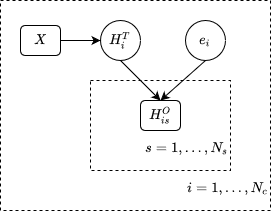
\includegraphics[width=0.4\linewidth]{entropy_ME.png}
	%
	\caption[DAG for the measurement error model of entropy.]%
	{DAG for the measurement error model of entropy. Circles represent latent variables, squares observed values or covariates, and large squares the nesting within specific units.}
	\label{fig:entropy_ME}
\end{figure}
%

\textcolor{red}{(in process)} \\

\begin{comment}
	Identification of model:  
	soft identification (see \citet{Depaoli_2021}) 
	
	- Normal measurement error model: 
	entropy_j ~ N( entropy_true_j, sigma_e) 
	
	- In (Faes_et_al_2021) they use a random effects model for the entropy. 
	entropy_j = entropy_true_j + error 
	error ~ N( 0, sigma_e) 
	* Notice both are the same (priors for entropy_true_j are needed) 
	
	- Beta measurement error model: 
	entropy_j ~ beta(alpha, beta) 
	alpha = mu*M        ->  mu = alpha / M (mean) 
	beta = (1 - mu)*M  ->  M = alpha + beta (prior sample size) 
	* where mu = entropy_true_j and M is a distribution centered in 10 (utterances) 
\end{comment}
%
%
\noindent \textbf{Measurement models for the CJ and HJ procedures:} \\
%
\textcolor{red}{(in process)}

\begin{comment}
	
	Considering the intelligibility of any stimulus is determined by three interrelated parties: the message, speaker, and listener, and that the inherent variability within each integrating part could be high, the current research assumes the utterances are equivalent among each other.
	
	It will consider the correlation with the entropy measure.
	%
	\begin{enumerate}
		\item \textbf{Dichotomous CJ (CJ-D):} the Bradley-Terry-Luce model (BTL) \citep{Bradley_et_al_1952, Luce_1959}, used when the comparative judgments are dichotomous (CJ-D), 
		%
		\item \textbf{Ordinal CJ (CJ-O):} the Generalized Bradley-Terry-Luce model BTL(k) \citep{Tutz_1986, Agresti_1992}, used when the comparative ordinal CJ (CJ-O).
		%
		\item \textbf{Absolute (holistic) judgments (HJ):}
	\end{enumerate}
\end{comment}
%
%